% XeLaTeX can use any Mac OS X font. See the setromanfont command below.
% Input to XeLaTeX is full Unicode, so Unicode characters can be typed directly into the source.

% The next lines tell TeXShop to typeset with xelatex, and to open and save the source with Unicode encoding.

%!TEX TS-program = xelatex
%!TEX encoding = UTF-8 Unicode

\documentclass[12pt]{article}
\usepackage{geometry}                % See geometry.pdf to learn the layout options. There are lots.
\geometry{letterpaper}                   % ... or a4paper or a5paper or ... 

\geometry{left=1in}
\geometry{right=1in}
\geometry{bottom=1.9in}
\geometry{top=1in}

%
%Setting the font
%
\usepackage{times}

%
%Rotating tables (e.g. sideways when too long)
%
\usepackage{rotating}

%
%For multiple rows in tables
%
\usepackage{multirow}

% 
%Line numbering in verse environment
%
\usepackage{lineno} 

%
%Fancy-header package to modify header/page numbering (insert last name)
%
\usepackage{fancyhdr}
\pagestyle{fancy}
\lhead{} 
\chead{} 
\rhead{Quan \thepage} 
\lfoot{} 
\cfoot{} 
\rfoot{} 
\renewcommand{\headrulewidth}{0pt} 
\renewcommand{\footrulewidth}{0pt} 
%To make sure we actually have header 0.5in away from top edge
%12pt is one-sixth of an inch. Subtract this from 0.5in to get headsep value
\setlength{\headsep}{1in}

\usepackage{setspace}
\doublespacing

\usepackage{booktabs}
\usepackage[american]{babel}
\usepackage{csquotes}
\usepackage[style=mla]{biblatex}
\usepackage{url}
\usepackage[parfill]{parskip}
\usepackage{listings}
 \usepackage{float}

\usepackage{titlesec}
\usepackage{amsmath}
\usepackage{amssymb}

\usepackage{xcolor}

\lstset{language=python}
\lstset{breaklines}
\definecolor{mygreen}{rgb}{0,0.6,0}
\definecolor{mygray}{rgb}{0.5,0.5,0.5}
\definecolor{mymauve}{rgb}{0.58,0,0.82}

\lstset{numbers=left, 
numberstyle=\tiny, 
keywordstyle=\color{blue},
commentstyle=\color{mygreen},    % comment style
rulecolor=\color{black},
frame=shadowbox, 
rulesepcolor=\color{red!20!green!20!blue!20},
stringstyle=\color{mymauve},     % string literal style
title=\lstname,
showspaces=false,
showstringspaces=false
}

\title{}
\author{}
\date{}                                           % Activate to display a given date or no date

\addbibresource{bib.bib}
\begin{document}

\begin{flushleft}
%%%%First page name, class, etc
Shengjie Quan\\
Professor: Adam C. Champion\\
CSE 3461	 \\
\today \\
\end{flushleft}

%%%%Title
\begin{center}
Response to Homework 2
\end{center}

%%%%Changes paragraph indentation to 0.5in
\setlength{\parindent}{0.5in}

\begin{singlespace}

\begin{enumerate}

\item 
	\begin{itemize}
	\item[(a.)] Firstly we sum up the three numbers.
	\begin{equation*}
	01010011_2 + 01100110_2 = 10111001_2
	\end{equation*}
	\begin{equation*}
	10111001_2 + 01110100_2 = 00101101_2
	\end{equation*}
	We get the sum, $00101101_2$.
	Then inverting each digit, we get the one's compliment, $11010010_2$
	\item[(b.)] According to some reading found online, the purpose of using one's complement of sum rather than sum is because of performance consideration. Due to different architecture, a system could be either big endian or little endian when representing a number in memory. When having the checksum as the one's complement of sum, the system can then sum up the whole package (including the checksum) to see if all bits equal one or not. This process according to that reading found online is endian independent. Thus the system does not need to convert between endians, which boost the performance. Also simply take the sum will cause checking the checksum inevitably becoming an endian dependent process. Thus the sum checksum has performance disadvantage comparing to one's complement of sum checksum.
	\item[(c.)] As describe above, to check the correctness of a package the receiver will sum up the whole package (including the checksum) and see if the result is zero or not. Using the number given in the problem for example, the receiver will sum up the three number, $01010011_2 + 01100110_2 + 01110100_2 = 00101101_2$ and then add the checksum $00101101_2$ to it. If the result has all bits one, then the receiver will be convinced that there is no error. However, otherwise, the receiver will know that there must be errors.\\
	For 1-bit error, it is not possible for this process failed to detect an error. However in the case of 2-bits error, it may be the case that the 2 bits error somehow still make the summation being all bits one. For a simple example suppose there are three numbers to transmit, 00000000, 00000001, 00000010, the checksum of them would be 11111100. Suppose there are two bits got flipped and the numbers become 00000000, 00000000, 00000011. Summing these three numbers and the correct checksum up, we get 11111111, which will tells the receiver that the package is correct according to the procedure. However, it is obvious not the case.
	\end{itemize}
\item
	To avoid the problem in Figure 3.27, the sender window, $w$, must fulfill the relation of $w \leqslant \frac{k}{2}$. Let's consider the worst situation that packages with sequence $n$ to $n+w-1$ were sent (suppose the sequence number base of this transmission is $n$) and all ACKs for these packages from the receiver to the sender get lost. At this moment the receiver is exacting packages with sequence number from $n+w$ to $n+2w-1$. The sender will then begin to retransmit the package with sequence number $n$. Since there are in total $k$ sequence numbers and the counting is circular, thus, we need the sequence number space to hold at least two times the sender window size, which gives us $2w \leqslant k$. Thus we get $w \leqslant \frac{k}{2}$.
\item
	Since the receiver's next expected sequence number is $501$ and the window size is assumed to be $2$. The receiver should have sent out the ACKs for $500$ and $499$. Thus the sender's window fully depends on how many of these ACKs are received. There are four possibility. If none of the ACKs being received, then the sender's window will be [$499$, $500$]. If ACK for $500$ not received but ACK for $499$ is received, then the sender's window will be [$500$, $501$]. If ACK for $500$ is received but ACK for $499$ not received, then the sender's window will be [$499$, $500$] (the window will not move up until the ACK for its lower bound is received in GBN). If ACK for $500$ is received and ACK for $499$ is received, then the sender's window will be [$501$, $502$]. So, there are three possible range for sender's window [$499$, $500$], [$500$, $501$] and [$501$, $502$].
\item
	The receiver cannot be absolutely certain that no bit errors have occurred. An existing example is the 2-bits one in 1(c). Even for only 2 bits in the data got flipped, the checksum may still match the value expected. Thus the receiver cannot be absolutely certain that no bit errors have occurred even when checksum matches.
\item
	The problem for only using NAKs is that after receiving package $n$, the receiver need to wait until package $n+2$ arrives in order to know that the package $n+1$ is lost then it can send back a NAK (since the sender won't checking whether packages being received or not but will only retransmit lost package requested by the sender and the sender won't notice a package is lost until its successor being received). This may require long time for the lost package to be recovered when the data are not sent frequently.\\
	However, in the setting of the problem, if we assume a lot of data are sent and few of packages get lost. The problem mentioned above for using NAKs only protocol is negligible. Moreover, using NAKs only protocol can dramatically reduce the time for sending unnecessary feedback ACKs (since in the setting, not many packages get lost) and there are not many NAKs, which results in more bandwidth devoting into actual data transmission. Thus, the protocol can boost up the utility rate of the network. So, in the setting of the problem, a NAKs only protocol is preferable to using ACKs.
\item 
	For a traditional circular DHT with $N$ nodes since each node only track its two neighboring nodes, to find the node responsible for a key, all $N$ nodes may need to forward the request message and on average and on average, $\frac{N}{2}$ messages needs to be passed, which is in the order of linear time, $O(n)$. Thus, this traditional approach is slow. However, when we add shortcuts to the circular DHT, a node not only tracks the two neighboring nodes but also tracks a small number of selected peers. This concept is illustrated in the figure below. 
	\begin{figure}[h]
	\centering
	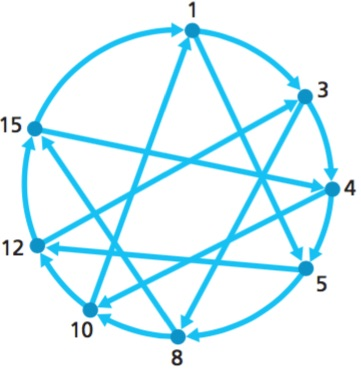
\includegraphics[width=0.3\textwidth]{6} 
	\end{figure}
	\\This approach allows the request to by pass some nodes by taking the shortcuts and reach the destination quicker (means a request being passed less times before it reach the node responsible for the key). For the example in the textbook, suppose peer 4 is ask about key 11, using the shortcut approach, peer 4 will forward the request to peer 10 and then peer 10 will forward the request to peer 12 who is the closest peer to key 11. However, using the traditional approach (without any shortcuts), peer 4 will need to forward the request to peer 5, then to 8, then to 10, and finally to 12. Thus, from this example, we can see that indeed using shortcuts in DHT accelerate the requesting process.
\item
	\begin{itemize}
	\item[(a.)] The claim is true because although Bob does not upload anything, BitTorrent has the mechanism (often refereed to as tit-for-tat according to th textbook) that one peer will be randomly picked and be sent chunks. So, Bob is still possible be picked and sent data. Thus, Bob can receive a complete copy of th file. However, since Bob does not upload anything (upload rate is zero), Bob definitely will not be compatible among peers. Thus Bob may experience slow transmission speed.
	\item[(b.)] Assuming all Bob controlled computers are free rider, and having a fixed possibility for each of the computer being picked, the possibility of these Bob controlled computers as a whole being picked will increase. Bob can simply combine the chunks received by each of these computers and combine them into one file. By doing this, Bob makes his free-riding more efficient.
	\end{itemize}
\item
	\begin{itemize}
	\item[(a.)] According to the man page for netstat, -a argument indicates to ``show the state of all sockets''. The sockets used by server processes are normally not shown. In another word, using -a argument force netstat to show both listerning and non-listening sockets.\\
	According to the man page for netstat, -p argument means to ``show the PID and name of the program to which each socket belongs''.
	I was attempting to connect the ftp server: ftp.gnu.org. Following is the netstat output corresponding to that connection.
	\begin{lstlisting}[basicstyle=\ttfamily\scriptsize]
Proto Recv-Q Send-Q Local Address           Foreign Address   State   PID/Program name             
tcp     0     0 beta.cse.ohio-state.e:48572 ftp.gnu.org:ftp ESTABLISHED   29223/ftp    
	\end{lstlisting}
	From the output we can see that ftp connection is built on TCP protocol. The local domain is beta.cse.ohio-state.edu with port 48572. We know that eta.cse.ohio-state.edu is pointing to IP 164.107.113.18 according to previous experience. So the local IP is 164.107.113.18. For the remote side the connection is to ftp.gnu.org with ftp port. We all know ftp uses port 21 but netstat does not give the information about the remote side IP address. Further looking up the domain using nslookup, we can know that the remote IP address is 208.118.235.20. The netstat output also reveal the information that the connection is established by the process with PID 29223 and its Program name is ftp which is the default ftp program of linux.

	\item[(b.)] Adding -s argument to ping, we force ping to send out packages with our designated data size. For example, by executing the command, ping -s 1024 www.google.com, we sent out 1052 (1024 + size of head) bytes each time to google's server.\\
	Adding -i argument to ping, we force ping to send out packages with out designated time interval (in the unit of second) in between. For example, by executing the command, ping -i 0.2 www.google.com, we sent out packages to google's server every 200ms.\\
	For the output of ping command, it consists of five pieces of information. The first one is the size of data responded. The second one is the address of the responder (domain name and/or IP). The third one is called icmp\_seq. It indicates the number of that package in the transmission. The forth one is ttl which means the time to live. During the transmission, each time the package pass though a router, its ttl got decremented. The package will get dropped when ttl reaches 0. The fifth one is time which tells the length of the time to send a ping package from the sender to the server and the server respond back to the sender.
	\end{itemize}
\end{enumerate}
\end{singlespace}

\clearpage

\printbibliography
\end{document}  